
% ---------------------------------------------------------------------------
% Algorithmic use cases: search, order finding, QAOA.  Generated data and
% figures come from code/implementation_3_algorithms (search_scaling.py,
% shor_walk.py, qaoa_walk.py, make_figures.py); numbers quoted below are
% read from the JSON files those scripts write.  Added 20 Sep 2026.
% ---------------------------------------------------------------------------
\subsection{Unstructured Search: the Square-Root Law and the Price of Constant Time}
\label{sec:res-search}

The search results serve one purpose in this thesis: to fix, by direct
simulation, what a walk can and cannot do for unstructured search, so that
the constant-time result of Dal Favero et al.~\cite{DalFavero_2024} cited in
Section~\ref{sec:search} is read correctly. Three models are simulated on the
complete graph $K_N$ with one marked vertex, all by exact state-vector
evolution: the coined discrete-time walk with the Grover coin and the
$-\mathbb{I}$ oracle coin at the marked vertex, which is the walk analogue of
Grover's algorithm~\cite{Grover_1996, Ambainis_2005}; the continuous-time walk
$H = -\gamma A - \ket{w}\bra{w}$ at the critical $\gamma = 1/N$ of Childs and
Goldstone~\cite{Childs_2004a}; and the nonlinear continuous-time walk of Meyer
and Wong~\cite{Meyer_2013}, $H = -\gamma A - \ket{w}\bra{w} - g\,|\psi(x)|^2$,
which is the single-species, cubic-only ancestor of the cubic--quintic
many-body construction in~\cite{DalFavero_2024}. For the nonlinear model the
hopping rate is kept on resonance as the state evolves, $\gamma(t) = (1 +
g|\psi_w|^2 - g|\psi_u|^2)/(N-2)$, which is the condition Meyer and Wong derive
for the reduced two-level dynamics; without it the nonlinearity detunes the
marked vertex and the search fails outright. The discrete-time walk is
implemented without matrices and cross-checked against the dense operator of
Section~\ref{sec:qiskittooling} for $N \leq 32$ to $10^{-10}$.

\paragraph*{Both linear walks obey the square-root law.}
Figure~\ref{fig:searchscaling}(a) gives the time to the first peak of the
success probability against $N$ from $4$ to $1024$. A power-law fit over
$N \geq 16$ gives $t \sim 0.94\,N^{0.52}$ for the coined walk and
$t \sim 1.573\,N^{0.500}$ for the continuous-time walk, the latter
indistinguishable from the analytic $(\pi/2)\sqrt{N}$. The coined walk's peak
success probability falls slowly with $N$, from $0.63$ at $N=32$ to $0.52$ at
$N = 1024$, consistent with the known $1/2$ limit on the complete graph, where
the continuous-time walk reaches unit probability. Neither model does better
than $\sqrt{N}$, and neither can: the bound of Bennett et
al.~\cite{Bennett_1997} applies to any linear unitary evolution with a
black-box oracle, and a walk is one. That is the whole of what a linear
discrete-time walk contributes to unstructured search, and it is why the
thesis claims no discrete-time analogue of the constant-time result.

\paragraph*{Constant time is bought with a nonlinearity that grows with $N$.}
Figure~\ref{fig:searchscaling}(b) is the nonlinear model at $g = 0.5N$, $N$
and $2N$. The time of the first peak is flat: at $g = 0.5N$ it moves from
$1.95$ at $N = 16$ to $2.22$ at $N = 1024$, a factor of $1.14$ over a
sixty-four-fold increase in $N$, while the linear walk's time grows by the
expected factor of eight. This reproduces, in the simplest possible setting,
the claim of~\cite{DalFavero_2024}: the search completes in $O(1)$ time.
Figure~\ref{fig:searchnonlinear} shows what that costs. Holding the target
time fixed at $t = 2$ and asking for the smallest $g$ that reaches success
probability $1/2$ gives $g_{\min}$ growing as $N^{1.27}$ over $N \in [16,
512]$ --- the resource that was time has become the strength of the
interaction, and it scales at least linearly with the size of the database.
In the many-body realisation of~\cite{DalFavero_2024} that strength is the
number of atoms in the condensate, and their statement that the particle
number must scale with $N$ is the same trade-off. The second cost is in
panel~(a): the full width at half maximum of the success peak shrinks as
$N^{-1/2}$, from $0.88$ to $0.13$ at $g = 0.5N$ and from $0.25$ to $0.03$ at
$g = 2N$, so the measurement must be timed to a precision that itself scales
with $\sqrt{N}$. This is exactly the difficulty the cubic--quintic tuning
in~\cite{DalFavero_2024} is designed to remove by widening the peak, and it is
absent from the linear walks, whose peak width is of the order of the run time.

The conclusion for this thesis is stated plainly. Constant-time search by a
quantum walk is a property of a nonlinear, and physically a many-body,
evolution; it is not available to the gate-model discrete-time walks used
everywhere else in this work, and it should not be read as a speed-up of the
walk primitive itself. The linear walks reproduce Grover's scaling to within
the fit error, and that is the result the later chapters build on.

\begin{figure}[htbp]
  \centering
  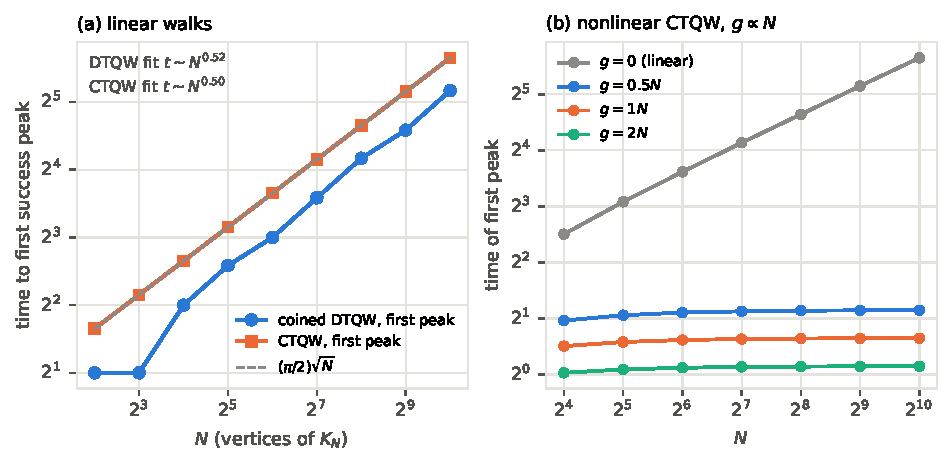
\includegraphics[width=\textwidth]{fig_search_scaling.pdf}
  \caption[Search by quantum walk on the complete graph]{Search on $K_N$ with
  one marked vertex. (a)~Time to the first success peak for the coined
  discrete-time walk and the continuous-time walk, with power-law fits over
  $N \geq 16$; both follow $\sqrt{N}$. (b)~The same quantity for the
  nonlinear continuous-time walk of Meyer and Wong with $g \propto N$: the
  time is constant in $N$.}
  \label{fig:searchscaling}
\end{figure}

\begin{figure}[htbp]
  \centering
  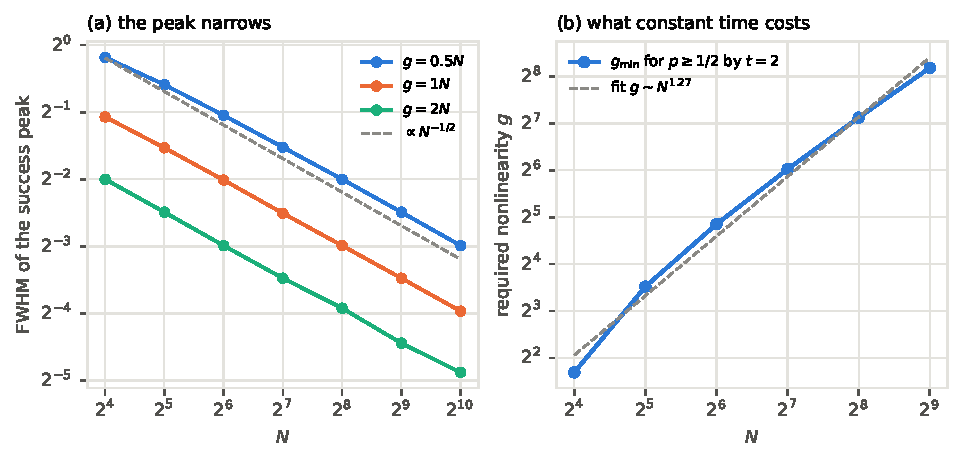
\includegraphics[width=\textwidth]{fig_search_nonlinear.pdf}
  \caption[The price of constant-time search]{What constant time costs in the
  nonlinear walk. (a)~Full width at half maximum of the success peak against
  $N$ at three values of $g/N$; the peak narrows as $N^{-1/2}$. (b)~The
  smallest nonlinearity that reaches success probability $1/2$ by $t = 2$,
  found by bisection; the fit gives $g_{\min} \sim N^{1.27}$.}
  \label{fig:searchnonlinear}
\end{figure}

\subsection{Order Finding as a Walk}
\label{sec:res-shor}

Section~\ref{sec:shor} set out what universality gives and does not give for
Shor's algorithm. The simulation here makes the structural half of that
statement concrete, and it is deliberately modest in what it claims. The
modular-multiplication operator $U_a\ket{x} = \ket{ax \bmod N}$ at the heart
of order finding is a permutation of the computational basis, and a
permutation of the basis is the one-step operator of a coinless quantum walk
on the directed graph whose arcs are $x \to ax \bmod N$. On the units of
$\mathbb{Z}_N$ that graph is a disjoint union of directed cycles, every cycle
length divides the order $r$ of $a$, and the cycle through $1$ has length
exactly $r$. Restricted to that cycle $U_a$ is the cyclic shift on
$\mathbb{Z}_r$, whose eigenphases are $2\pi k/r$: this is the sense in which
the walk on the cycle of Section~\ref{sec:prelim-dtqw} and the order-finding
unitary share their algebraic core, and it is the sense, and the only sense,
in which order finding is ``a walk'' here.

Table~\ref{tab:shor} and Figure~\ref{fig:shorwalk} give the result for nine
$(N, a)$ pairs with $N$ up to $35$. In every case the cycle decomposition of
the functional graph and the eigenphases of $U_a$ on the cycle through $1$ are
computed exactly and agree with $k/r$ to machine precision; that is a check
on the construction rather than a finding. Two things are then done with the
walk. The first is walk-native and slow: started at $\ket{1}$ and stepped,
the walker returns with probability one exactly when $r$ divides $t$
(Figure~\ref{fig:shorwalk}(a)), so the order can be read off the first
revival. This costs $r$ applications of $U_a$, which is exponential in
$\log N$ in the worst case and offers no advantage over classical trial
multiplication; it is included to show where the advantage is \emph{not}. The
second is Shor's own read-out: phase estimation on $U_a$ with $m = 2n$
counting qubits, built in Qiskit with the controlled powers $U_a^{2^j}$
synthesised as dense unitaries and sampled with Aer at 4096 shots. The
measured phases concentrate on $k/r$ (Figure~\ref{fig:shorwalk}(b)), and
continued fractions return the exact order in a fraction of shots between
$0.31$ and $0.51$, the remainder returning proper divisors of $r$ as Shor's
analysis predicts; the resulting factorisations are correct wherever
$a^{r/2} \not\equiv -1$, and for $N = 21$, $a = 5$ and $N = 33$, $a = 2$ the
run fails for exactly that arithmetic reason, not a simulation one.

What the table also records is the cost of treating $U_a$ as a walk step to be
synthesised rather than as modular arithmetic to be compiled. At $N = 15$ the
circuit needs $12$ qubits and some $520$ CX gates; at $N = 33$ and $35$ it
needs $18$ qubits and roughly $50{,}000$. The growth is that of dense
synthesis on $n$ target qubits, $\Theta(4^n)$, and it says nothing about
Shor's algorithm, whose modular exponentiation is polynomial in $n$ precisely
because it is \emph{not} synthesised from the permutation matrix. The
point of Section~\ref{sec:shor} is thereby confirmed from the other side:
the walk picture is a correct description of the order-finding operator and
its spectrum, and phase estimation on the walk factors $15$, $21$ and $35$
in simulation; but the walk picture is not a route to an efficient circuit,
and nothing here should be cited as one.

\begin{figure}[htbp]
  \centering
  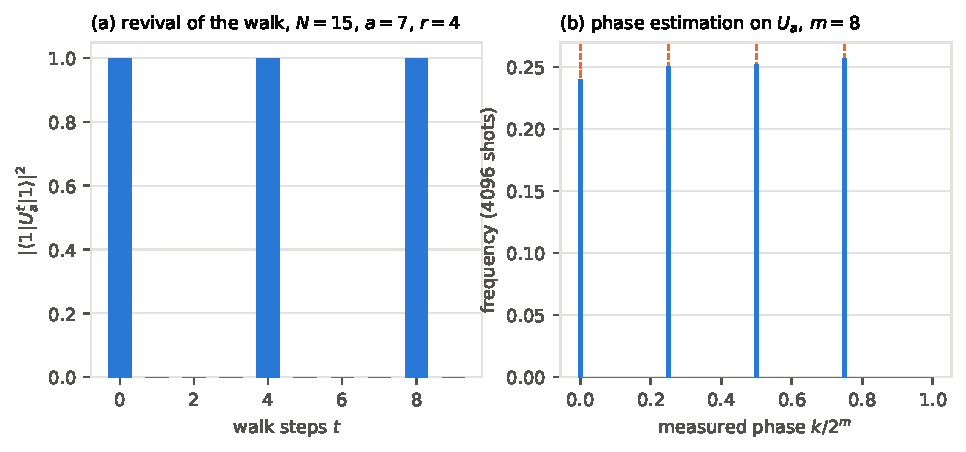
\includegraphics[width=\textwidth]{fig_shor_walk.pdf}
  \caption[Order finding on the permutation walk]{Order finding for $N = 15$,
  $a = 7$. (a)~Return probability of the walk $U_a$ started at $\ket{1}$; the
  revivals at multiples of $r = 4$ read the order at a cost of $r$ steps.
  (b)~Phase estimation on $U_a$ with $m = 8$ counting qubits, 4096 Aer shots;
  the measured phases sit at $k/4$ (dashed lines).}
  \label{fig:shorwalk}
\end{figure}

% Generated by make_figures.py -- do not edit by hand.
\begin{table}[htbp]
\centering\small
\caption{Order finding as phase estimation on the permutation walk $U_a$. Cycle lengths are those of $x \mapsto ax \bmod N$ on the units of $\mathbb{Z}_N$; $P(r)$ is the fraction of 4096 shots whose continued-fraction denominator is exactly $r$ (the remainder return divisors of $r$, as in Shor's analysis); depth and CX are for the transpiled circuit with $m = 2n$ counting qubits, basis $\{\mathrm{CX}, R_Z, \sqrt{X}, X\}$, with the controlled walk steps synthesised as dense unitaries.}
\label{tab:shor}
\begin{tabular}{rrrlrrrrl}
\hline
$N$ & $a$ & $r$ & cycles & $m$ & $P(r)$ & qubits & CX & factors \\
\hline
15 & 7 & 4 & 4, 4 & 8 & 0.51 & 12 & 522 & 3$\times$5 \\
15 & 2 & 4 & 4, 4 & 8 & 0.51 & 12 & 522 & 3$\times$5 \\
15 & 11 & 2 & 2, 2, 2, 2 & 8 & 0.50 & 12 & 292 & 5$\times$3 \\
15 & 4 & 2 & 2, 2, 2, 2 & 8 & 0.50 & 12 & 289 & 3$\times$5 \\
21 & 2 & 6 & 6, 6 & 10 & 0.31 & 15 & 10103 & 7$\times$3 \\
21 & 5 & 6 & 6, 6 & 10 & 0.31 & 15 & 10103 & --- \\
21 & 8 & 2 & 2, 2, 2, 2, 2, 2 & 10 & 0.50 & 15 & 1094 & 7$\times$3 \\
33 & 2 & 10 & 10, 10 & 12 & 0.39 & 18 & 49779 & --- \\
35 & 3 & 12 & 12, 12 & 12 & 0.32 & 18 & 49739 & 7$\times$5 \\
\hline
\end{tabular}
\end{table}


\subsection{Walk Mixers for the Quantum Approximate Optimisation Algorithm}
\label{sec:res-qaoa}

Of the three algorithmic use cases this is the one where the walk changes the
answer rather than describes it. The problem is balanced Max-Cut, or graph
bisection: maximise the weighted cut of a graph on $n = 8$ vertices subject to
$|S| = 4$. The constraint is what matters. The feasible strings are those of
Hamming weight four, and they are the vertices of the Johnson graph $J(8,4)$,
seventy in number, two adjacent when they differ by one transposition. Three
mixers are compared with the same cost layer $e^{-i\gamma C}$, the same
depths $p = 1$ to $4$, and the same optimiser, COBYLA from twelve random
starts with the best kept~\cite{Farhi_2014, Hadfield_2019}. The transverse-field
mixer $e^{-i\beta\sum_j X_j}$ is, as Section~\ref{sec:optimisation} noted, a
continuous-time walk on the hypercube; it does not respect the constraint, so
it is paired with a quadratic penalty $\lambda(\sum_j z_j - 4)^2$ in the
cost. The continuous-time walk mixer $e^{-i\beta A_J}$ on the Johnson graph is
the construction of Marsh and Wang~\cite{Marsh_2019, Marsh_2020}, identical to
the complete $XY$ mixer of Hadfield et al.; it cannot leave the feasible
subspace. The discrete-time mixer applies one coined walk step on the Johnson
graph per layer, $W(\beta) = S\,(\mathbb{I} \otimes e^{-i\beta G})$ with $G$
the Grover coin on a sixteen-dimensional coin register that is traced out at
the end; it is feasibility preserving for the same reason. The figure of merit
is the expected cut of a feasible outcome, $\mathbb{E}[C(x)\,\mathbb{1}_{x
\text{ feasible}}]/C_{\mathrm{opt}}$, so that an infeasible answer scores
zero, which is the value it has.

\paragraph*{The constraint-respecting walks win, and by a margin that has
nothing to do with optimisation quality.}
Table~\ref{tab:qaoa} and Figure~\ref{fig:qaoamixers} give the result over six
random weighted instances. The continuous-time Johnson-graph mixer reaches a
ratio of $0.85 \pm 0.02$ at $p=1$ and $0.91 \pm 0.02$ at $p=4$, with every
sampled string feasible. The penalised $X$ mixer reaches $0.31 \pm 0.07$ at
$p=1$ and never exceeds $0.38$, and the reason is not that it finds poor cuts:
conditioned on feasibility its cuts score $0.75$ to $0.85$, close to the walk
mixers. It simply returns an infeasible string more than half the time, and
the penalty, whatever its weight, does not repair this within four layers.
The walk on the feasible graph removes the problem rather than penalising it,
which is the argument Marsh and Wang make and which this simulation
reproduces.

\paragraph*{The discrete-time mixer works, but one step per layer is a weak
mixer.}
The coined mixer reaches $0.76 \pm 0.02$ at $p = 1$ and $0.86 \pm 0.05$ at
$p = 4$: always above the $X$ mixer, always feasible, and always below the
continuous-time walk on the same graph. Its $p=1$ figure deserves a plain
statement: a uniform draw from the feasible set already scores $0.76$ on
these instances, so at one layer the discrete-time mixer does no better than
random feasible guessing. The reason is not hard to see. One coined step moves
amplitude only to adjacent vertices of $J(8,4)$, whereas $e^{-i\beta A_J}$
couples all vertices at once, and a single coin angle is a poorer
parametrisation of mixing than a single continuous time. By $p = 4$ the
discrete-time mixer has recovered most of the gap, and the trend suggests
that more steps per layer, or a coin angle per step, would close it --- but
that experiment was not run and the claim is not made. For the register
count the comparison is not free either: the coined mixer carries four extra
qubits of coin. What the result establishes is narrower and sufficient for
the thesis: a discrete-time walk on the constraint graph is a legitimate QAOA
mixer, it inherits the feasibility guarantee of the continuous-time
construction, and its cost is a modest loss of mixing power per layer.

\begin{figure}[htbp]
  \centering
  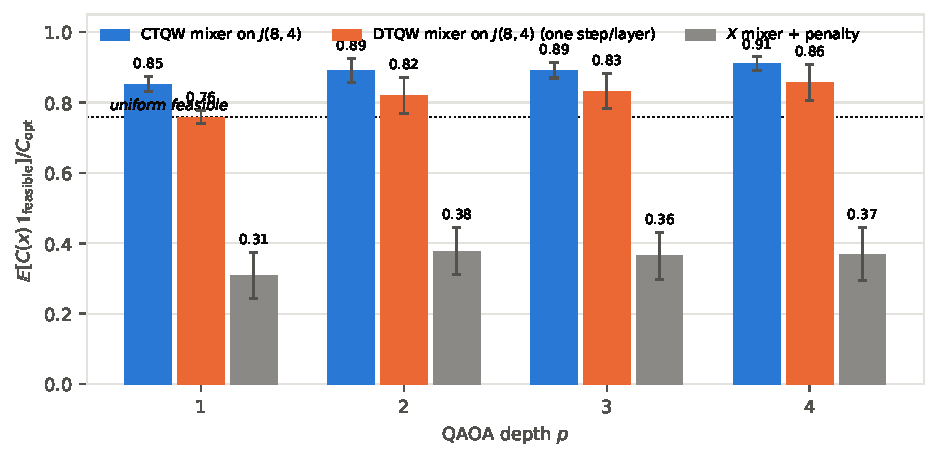
\includegraphics[width=\textwidth]{fig_qaoa_mixers.pdf}
  \caption[QAOA with walk mixers on balanced Max-Cut]{Balanced Max-Cut on six
  random weighted graphs ($n=8$, $|S|=4$). Bars give the mean over instances
  of the expected cut of a feasible outcome relative to the optimum, with the
  standard deviation over instances; the dotted line is the score of a
  uniform draw from the feasible set. Both walk mixers on the Johnson graph
  are feasibility preserving; the $X$ mixer with penalty is not.}
  \label{fig:qaoamixers}
\end{figure}

% Generated by make_figures.py -- do not edit by hand.
\begin{table}[htbp]
\centering\small
\caption[Balanced maximum cut: walk mixers against the penalised $X$ mixer]{Balanced Max-Cut on six random weighted graphs ($n=8$, $|S|=4$): approximation ratio $\mathbb{E}[C(x)\mathbb{1}_{\mathrm{feasible}}]/C_{\mathrm{opt}}$ and probability of a feasible outcome, mean $\pm$ s.d.\ over instances, best of twelve COBYLA starts. A uniform draw from the feasible set scores 0.76.}
\label{tab:qaoa}
\begin{tabular}{clrr}
\hline
$p$ & Mixer & Ratio & $P(\mathrm{feasible})$ \\
\hline
1 & CTQW mixer on $J(8,4)$ & $0.852 \pm 0.022$ & $1.00 \pm 0.00$ \\
 & DTQW mixer on $J(8,4)$ (one step/layer) & $0.759 \pm 0.018$ & $1.00 \pm 0.00$ \\
 & $X$ mixer + penalty & $0.308 \pm 0.066$ & $0.38 \pm 0.07$ \\
\hline
2 & CTQW mixer on $J(8,4)$ & $0.891 \pm 0.035$ & $1.00 \pm 0.00$ \\
 & DTQW mixer on $J(8,4)$ (one step/layer) & $0.820 \pm 0.050$ & $1.00 \pm 0.00$ \\
 & $X$ mixer + penalty & $0.378 \pm 0.067$ & $0.48 \pm 0.08$ \\
\hline
3 & CTQW mixer on $J(8,4)$ & $0.892 \pm 0.022$ & $1.00 \pm 0.00$ \\
 & DTQW mixer on $J(8,4)$ (one step/layer) & $0.833 \pm 0.051$ & $1.00 \pm 0.00$ \\
 & $X$ mixer + penalty & $0.364 \pm 0.067$ & $0.45 \pm 0.08$ \\
\hline
4 & CTQW mixer on $J(8,4)$ & $0.910 \pm 0.020$ & $1.00 \pm 0.00$ \\
 & DTQW mixer on $J(8,4)$ (one step/layer) & $0.857 \pm 0.051$ & $1.00 \pm 0.00$ \\
 & $X$ mixer + penalty & $0.370 \pm 0.077$ & $0.47 \pm 0.10$ \\
\hline
\end{tabular}
\end{table}


